\documentclass[a4paper]{article}

% Language and font encodings
\usepackage[english]{babel}
\usepackage[utf8x]{inputenc}
\usepackage[T1]{fontenc}
\usepackage[a4paper,top=3cm,bottom=2cm,left=3cm,right=3cm,marginparwidth=1.75cm]{geometry}
\usepackage{titling}
\usepackage{amsmath}
\usepackage{titlesec}
\usepackage{graphicx}
\usepackage{tabularx}
\usepackage[colorinlistoftodos]{todonotes}
\usepackage[colorlinks=true, allcolors=blue]{hyperref}
\usepackage{fancyhdr}
\usepackage{wrapfig}
\usepackage{subcaption}

\graphicspath{{images/}}

\title{Cosmology Assignment 2}
\author{Daniel Herman: daniel.herman@astro.uio.no}

\begin{document}

\begin{titlepage}
\maketitle
\end{titlepage}

(Code included for exercises 1 and 2 at \url{https://github.com/hermda02/Cosmology-Assignment-2})

\textbf{Exercise 1.}
Compute and plot the Fourier conjugate of the top-hat smoothing function where $W(x) = 1$ when $x \leq |R|$ and $W(x) = 0$ elsewhere. 

The computed Fourier transform is plotted in figure \ref{fig:mesh1}. The number of harmonics and FWHM of the transform are shown on the plots.

\begin{figure}[h]
\centering
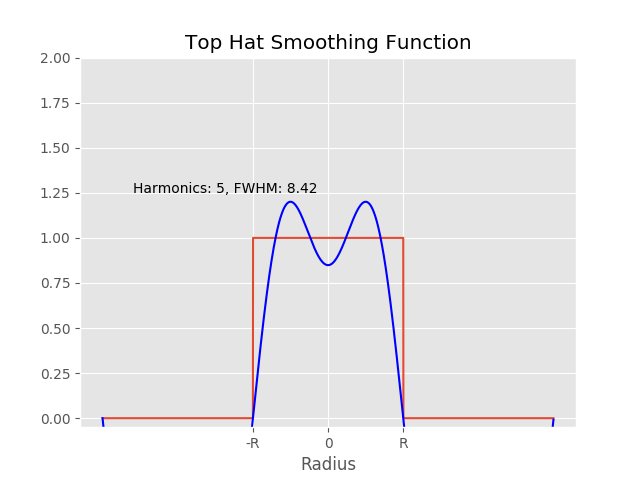
\includegraphics[scale=0.45]{exercise1_5harm}
\end{figure}

\begin{figure}[h]
\centering
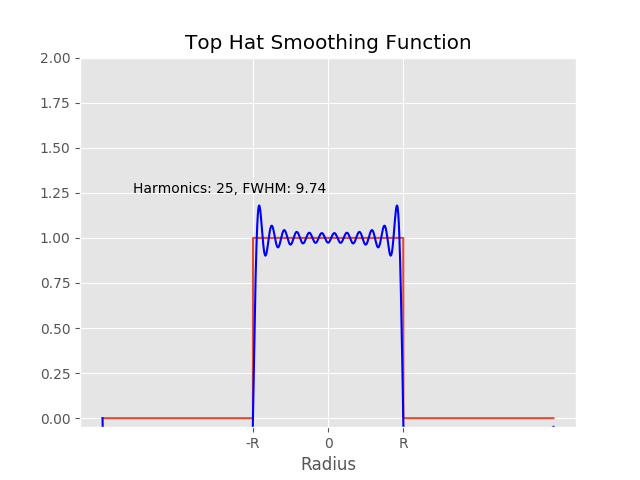
\includegraphics[scale=0.45]{exercise1_25harm}
\end{figure}

\begin{figure}[h]
\centering
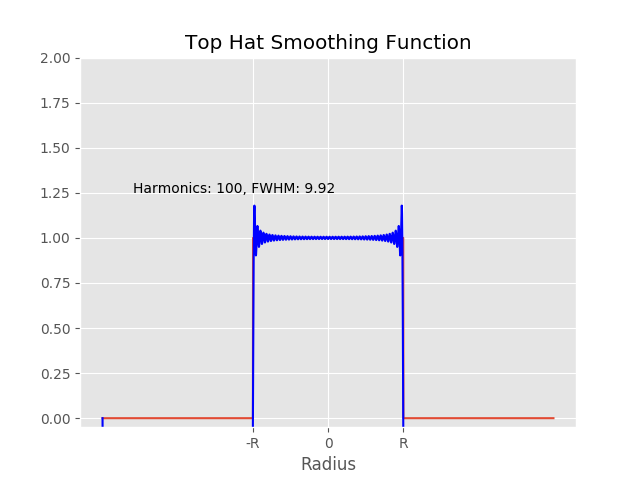
\includegraphics[scale=0.45]{exercise1_100harm}
\caption{The Fourier transform of the top-hat for 5, 25, and 100 harmonics}
\label{fig:mesh1}
\end{figure}

\clearpage

\textbf{Exercise 2.}

To numerically solve the overdensity random walk, we utilize a recursive algorith where the probability distribution we draw from changes with the smoothing factor $S_c$, which we decrease by $\epsilon$ at the end of each step.  We define $S_c = 2 \pi / k$ and $\sigma^2(S_c) = \pi / S_c^4$ where $\sigma^2(S_c)$ is the variance of the function $P(k)=k$. We start with a radius $S_c$ such that $\sigma^2(S_c) < 10^{-4}$. So, we start with $k = 0.47$, giving us an inital $S_c = 13.368$. We set $\epsilon = 0.03$. We stop taking random steps when $S_c = 1.0$, or after 4000 steps. We see the densities in figure. The probability distribution as given in equation \ref{eq:1} is over-plotted for comparison.

\begin{figure}[h]
\centering
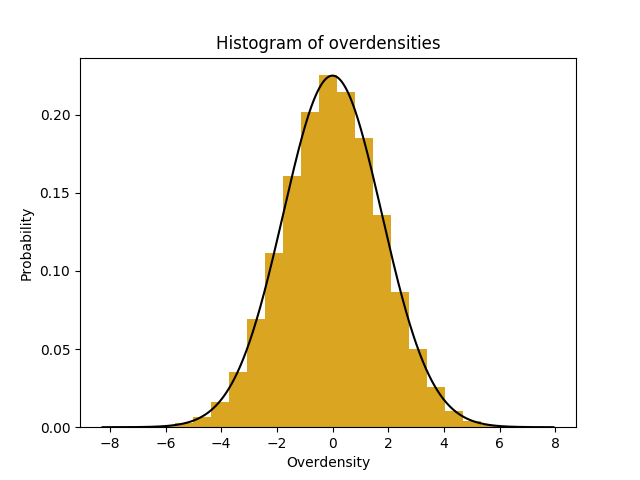
\includegraphics[scale=0.475]{densityhisto}
\caption{The over/under-densities for $10^5$ random walks with $k=0.47$ and $\epsilon = 0.03$.}
\end{figure}

\begin{equation}
P(\delta|M) = \dfrac{1}{\sqrt{2 \pi}\sigma(M)}\exp \Big[ - \dfrac{\delta^2}{2\sigma^2(M)} \Big]
\label{eq:1}
\end{equation}

Removing all random walks where $\delta$ becomes greater than $\delta_{crit}$ at any point along the walk, we see the following histogram of final $\delta$ values. The analytical expression for the distribution shown for $\delta$ provided that $\delta$ was never larger than $\delta_{crit}$ is given by equation \ref{eq:2} and is over-plotted for comparison.

\begin{figure}[h]
\centering
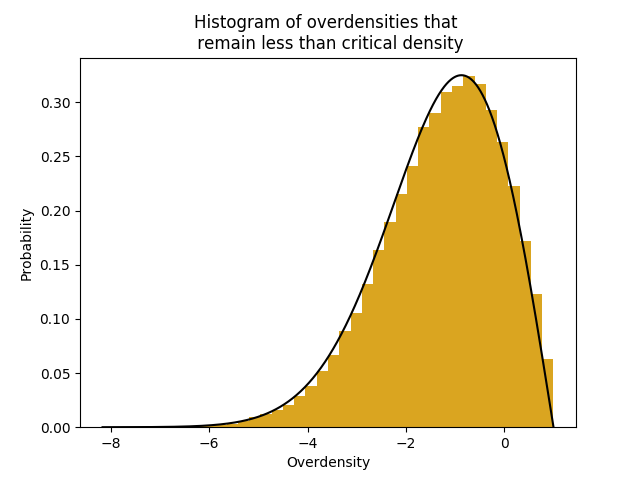
\includegraphics[scale=0.475]{undercrit}
\caption{All random walks in which $\delta$ is less than $\delta_{crit}$ for every step.}
\end{figure}

\begin{equation}
P_{nc}(\delta|M) = P(\delta|M) - P([2\delta_{crit} - \delta]|M) = \dfrac{1}{\sqrt{2 \pi}\sigma(M)} \Big( \exp \Big[ - \dfrac{\delta^2}{2\sigma^2(M)} \Big] - \exp \Big[ - \dfrac{[2\delta_{crit}-\delta]^2}{2\sigma^2(M)} \Big] \Big)
\label{eq:2}
\end{equation}
\clearpage

\textbf{Exercise 3.}

(1) We see in Exercise 2 that the probability that any perturbation never becomes greater than $\delta_{crit}$ is given by the difference between the two probability distribution functions (PDFs). For a mass at point \textbf{x} to be embedded within a collapsed object of mass > $M$, the mass at \textbf{x} must be in an overdense region, where $\delta > \delta_{crit}$. Therefore, the probability $P(\delta > \delta_{crit} | M) = P(>M)$ is equal to all the probability for all possible values of $\delta$ (1) subtracted by the total probability that $\delta$ is never greater than $\delta_{crit}$ (given by the integral over $\delta$ of equation \ref{eq:2}). So we see:

\begin{equation}
P(>M) = 1 - \int_{-\infty}^{\delta_{crit}} d \delta P_{nc}(\delta|M)
\label{eq:3}
\end{equation}

The probability that a mass at \textbf{x} is within a collapsed object of mass $M$ is the total probability of all $\delta$'s given mass $M$ (i.e. 1) minus the probability that all $\delta$'s given a mass $M$ never reach a value greater than $\delta_{crit}$. If a $\delta$ becomes greater than $\delta_{crit}$, then that $\delta$ will collapse, or be a part of a collapsed object. As an expression, this becomes

\begin{equation}
P(>M) = 1 - \int_{-\infty}^{\delta_{crit}} d\delta P_{nc}(\delta|M)
\end{equation}

(2) Show that: $P(>M) = 2P(\delta > \delta_{crit}|M) = 1 - $erf$(\nu/\sqrt{2})$ where $\nu = \delta / \sigma(M)$.

\begin{align*}
P(>M) =& 1 - \int_{-\infty}^{\delta_{crit}} d\delta P_{nc}(\delta|M) =  P(\delta > \delta_{crit}|M) \\
=& 1 - P_{nc}(\delta < \delta_{crit}|M)\\
=& 1 - P(\delta<\delta_{crit}|M) - P([2\delta_{crit} - \delta]<\delta_{crit}|M) \\
=& 1 - (P(\delta<\delta_{crit}|M) - P([\delta_{crit} - \delta]<0|M)) \\
=& 1 - (P(\delta<\delta_{crit}|M) - P(\delta>\delta_{crit}|M)) \\
=& 1 - (1 - P(\delta>\delta_{crit}|M)) + P(\delta>\delta_{crit}|M) \\
=& 2P(\delta>\delta_{crit}|M) \\ 
=& 2(\dfrac{1}{\sqrt{2 \pi}\sigma(M)}) \Big(\int_{0}^{\infty} d\delta e^{ - \dfrac{\delta^2}{2\sigma^2(M)}} - \int_{\delta_{crit}}^{\infty} d \delta e^{ - \dfrac{\delta^2}{2\sigma^2(M)}} \Big) \\
\end{align*}
The last line of the above expression is brings us to
\begin{equation}
1 - erf(\nu/\sqrt{2})
\end{equation}



\end{document}